\documentclass[aspectratio=169]{beamer}

\usetheme{Madrid}
\usecolortheme{default}
\usepackage{tikz}
\usepackage{pgfplots}

\pgfplotsset{compat=1.18}
\usepackage{amsmath}
\usepackage{amssymb}
\usepackage{booktabs}
\usepackage{array}

\title{Statistics}
\subtitle{Descriptive and Frequentist Statistics}
\author{GAYATHRI P S}

\begin{document}

\begin{frame}
\titlepage
\end{frame}

\begin{frame}{Statistics}
\textbf{Definition:}

Statistics is the branch of mathematics concerned with the
\textbf{collection, organization, analysis, interpretation, and
presentation of data} to obtain useful conclusions and support
decision-making.

\vspace{0.4cm}

\textbf{In simple words:}

Statistics helps us convert raw data into meaningful information
and knowledge for making decisions.

\vspace{0.4cm}

\begin{block}{Two Major Areas}
\begin{itemize}
    \item Descriptive Statistics
    \item Inferential Statistics
\end{itemize}
\end{block}

Frequentist statistics is one important framework for statistical
inference.
\end{frame}

\begin{frame}{Data, Information, Knowledge and Intelligence}

\begin{center}
\Large
\textbf{Data}
$\rightarrow$
\textbf{Information}
$\rightarrow$
\textbf{Knowledge}
$\rightarrow$
\textbf{Intelligence}
\end{center}

\vspace{0.5cm}

\begin{itemize}
    \item \textbf{Data:} Raw facts, observations, measurements or values.
    \item \textbf{Information:} Processed and organized data that has meaning.
    \item \textbf{Knowledge:} Understanding obtained by interpreting information using context, rules and experience.
    \item \textbf{Intelligence:} Ability to use knowledge for reasoning, problem-solving, planning and decision-making.
\end{itemize}
\end{frame}

\begin{frame}{Example: From Data to Intelligence}

Suppose student marks are:

\[
10,\;12,\;15,\;15,\;18,\;20,\;25
\]

\begin{enumerate}
    \item \textbf{Data:} The raw marks.
    \item \textbf{Information:} Average mark, highest mark, lowest mark, etc.
    \item \textbf{Knowledge:} Understanding whether student performance is improving or declining.
    \item \textbf{Intelligence:} Identifying weak areas and recommending suitable topics for additional practice.
\end{enumerate}

\vspace{0.3cm}

\begin{center}
\textbf{Data provides the raw material $\rightarrow$ Intelligence supports action.}
\end{center}
\end{frame}

\begin{frame}{Artificial Intelligence}

\textbf{Definition:}

Artificial Intelligence (AI) is a branch of computer science that
develops systems capable of performing tasks that normally require
human intelligence.

\vspace{0.3cm}

Examples of such activities include:

\begin{itemize}
    \item Learning
    \item Reasoning
    \item Problem-solving
    \item Planning
    \item Decision-making
    \item Perception
    \item Content generation
\end{itemize}

\vspace{0.3cm}

\begin{block}{AI and Statistics}
AI systems use \textbf{data and algorithms} to learn patterns,
make predictions, reason about problems and perform intelligent tasks.
\end{block}
\end{frame}

\begin{frame}{Humans and AI}

\begin{center}
\begin{tabular}{>{\bfseries}m{4cm} m{5.5cm}}
\toprule
Humans & AI Systems \\
\midrule
Natural intelligence & Artificial intelligence \\
Human abilities & Algorithms and computational models \\
Learn from experience & Learn patterns from data \\
Use knowledge and experience & Use learned patterns and models \\
Reason and make decisions & Perform computational reasoning and decision-making \\
Biological brain & Computer systems \\
\bottomrule
\end{tabular}
\end{center}

\vspace{0.4cm}

\begin{center}
\textbf{Humans: Abilities + Knowledge}

\textbf{AI: Algorithms + Data}
\end{center}
\end{frame}

\begin{frame}{Human-like Activities Performed by AI}

\begin{center}
\Large
\textbf{ARTIFICIAL INTELLIGENCE}
\end{center}

\vspace{0.3cm}

\begin{center}
\begin{tabular}{c c c c}
\textbf{Think} & \textbf{Plan} & \textbf{Reason} & \textbf{Act} \\
Analyze patterns & Choose steps & Evaluate alternatives & Perform action
\end{tabular}
\end{center}

\vspace{0.5cm}

\begin{center}
\[
\boxed{
\text{Data + Algorithms}
\rightarrow
\text{Learning}
\rightarrow
\text{Reasoning}
\rightarrow
\text{Action}
}
\]
\end{center}

AI does not necessarily possess human intelligence in the same
sense as humans; rather, it is designed to perform or simulate
specific intelligent activities.
\end{frame}

\begin{frame}{Main Processes of AI}

Three important applications of AI are:

\begin{block}{1. Decision Making}
AI analyzes data and selects an appropriate option or action.
\end{block}

\begin{block}{2. Optimization}
AI searches for the best or most suitable solution among many
possible solutions.
\end{block}

\begin{block}{3. Content Generation}
AI generates new text, images, audio, video, code and other content
based on learned patterns.
\end{block}
\end{frame}

\begin{frame}{Descriptive Statistics}

\textbf{Definition:}

Descriptive statistics is concerned with organizing, summarizing and
presenting data in a meaningful form.

\vspace{0.4cm}

Major topics include:

\begin{itemize}
    \item Measures of central tendency
    \item Measures of dispersion
    \item Interquartile Range (IQR)
    \item Box plots
    \item Outliers
    \item Histograms
    \item Skewness
    \item Kurtosis
    \item Sample mean and variance
    \item Order statistics
    \item Sample covariance
    \item Sample covariance matrix
\end{itemize}
\end{frame}

\begin{frame}{Measures of Central Tendency}

Central tendency describes the \textbf{central or typical value}
of a dataset.

\begin{enumerate}
    \item Mean
    \item Median
    \item Mode
\end{enumerate}

\vspace{0.3cm}

For example:

\[
10,\;12,\;15,\;15,\;18
\]

\begin{itemize}
    \item Mean = 14
    \item Median = 15
    \item Mode = 15
\end{itemize}
\end{frame}

\begin{frame}{Mean}
The arithmetic mean is obtained by adding all observations and
dividing by the number of observations.
\[
\boxed{
\bar{x}=\frac{1}{n}\sum_{i=1}^{n}x_i
}
\]
Example:
\[
10,\;12,\;15,\;15,\;18
\]
\[
\bar{x}
=
\frac{10+12+15+15+18}{5}
=
14
\]
\begin{block}{Advantages}
Uses every observation and is easy to calculate.
\end{block}
\begin{alertblock}{Limitation}
The mean is sensitive to extreme values or outliers.
\end{alertblock}
\end{frame}

\begin{frame}{Median}

The median is the middle value after arranging observations
in ascending or descending order.

For an odd number of observations:

\[
10,\;12,\;15,\;18,\;20
\]

\[
\boxed{\text{Median}=15}
\]

For an even number of observations:

\[
10,\;12,\;15,\;18
\]

\[
\text{Median}
=
\frac{12+15}{2}
=
13.5
\]

The median is less affected by outliers than the mean.
\end{frame}

\begin{frame}{Mode}

The mode is the value that occurs most frequently.

Example:

\[
10,\;12,\;15,\;15,\;18,\;20
\]

Since 15 occurs twice:

\[
\boxed{\text{Mode}=15}
\]

A dataset may be:

\begin{itemize}
    \item Unimodal -- one mode
    \item Bimodal -- two modes
    \item Multimodal -- multiple modes
    \item Without a mode
\end{itemize}
\end{frame}

\begin{frame}{Measures of Dispersion}

Dispersion describes how widely the observations are spread
around the center.

Important measures:

\begin{itemize}
    \item Range
    \item Variance
    \item Standard deviation
    \item Interquartile range
\end{itemize}

\begin{block}{Range}
\[
\boxed{
\text{Range}=\text{Maximum}-\text{Minimum}
}
\]
\end{block}

Example:

\[
10,\;12,\;15,\;18,\;20
\]

\[
\text{Range}=20-10=10
\]
\end{frame}
\begin{frame}{Population Variance}
\begin{block}{Definition}
Population variance measures the average squared deviation of
each observation from the population mean.
\end{block}
\vspace{0.2cm}
For a population
\[
X=\{x_1,x_2,\ldots,x_N\}
\]
the population mean is
\[
\mu=\frac{1}{N}\sum_{i=1}^{N}x_i
\]
and the population variance is
\[
\boxed{
\sigma^2=
\frac{1}{N}\sum_{i=1}^{N}(x_i-\mu)^2
}
\]
\vspace{0.3cm}
\begin{exampleblock}{Example}
Consider the population
\[
X=\{2,4,6,8,10\}
\]
\[
\mu=\frac{2+4+6+8+10}{5}=6
\]
\[
\sigma^2=
\frac{(2-6)^2+(4-6)^2+(6-6)^2+(8-6)^2+(10-6)^2}{5}
\]
\[
\boxed{\sigma^2=\frac{40}{5}=8}
\]
\end{exampleblock}
\end{frame}
\begin{frame}{Population Standard Deviation}
\begin{block}{Definition}
Population standard deviation measures the typical spread of
observations around the population mean.
\end{block}

\vspace{0.2cm}
The population standard deviation is the positive square root
of the population variance:
\[
\boxed{
\sigma=
\sqrt{\frac{1}{N}\sum_{i=1}^{N}(x_i-\mu)^2}
}
\]
Equivalently,
\[
\boxed{\sigma=\sqrt{\sigma^2}}
\]
\vspace{0.3cm}
%\begin{exampleblock}{Example}
%For the population
%\[
%X=\{2,4,6,8,10\}
%\]
%from the previous slide,
%\[
%\sigma^2=8
%\]
%Therefore,
%\[
%\sigma=\sqrt{8}
%\]
%\[
%\boxed{\sigma\approx2.83}
%\]
%\end{exampleblock}
%\vspace{0.2cm}
%\begin{columns}
%\begin{column}{0.48\textwidth}
%\centering
%\textbf{Variance}
%\[
%\sigma^2=8
%\]
%Squared units
%\end{column}
%\begin{column}{0.48\textwidth}
%\centering
%\textbf{Standard Deviation}
%\[
%\sigma\approx2.83
%\]
%Same units as the data
%\end{column}
%\end{columns}
\end{frame}

\begin{frame}{Interquartile Range (IQR)}

The Interquartile Range measures the spread of the
middle 50\% of the data.

\[
\boxed{
IQR=Q_3-Q_1
}
\]

where:

\begin{itemize}
    \item $Q_1$ = First quartile
    \item $Q_3$ = Third quartile
\end{itemize}

Example:

\[
Q_1=15,\qquad Q_3=25
\]

Therefore:

\[
IQR=25-15=10
\]

IQR is relatively resistant to extreme observations.
\end{frame}

\begin{frame}{Box Plot}

A box plot summarizes data using five important values:

\begin{enumerate}
    \item Minimum
    \item First quartile ($Q_1$)
    \item Median
    \item Third quartile ($Q_3$)
    \item Maximum
\end{enumerate}

\begin{center}
\[
\text{Minimum}
\quad
\underbrace{
\boxed{
Q_1\quad|\quad Median\quad|\quad Q_3
}
}_{\text{Middle 50\%}}
\quad
\text{Maximum}
\]
\end{center}

The box represents the \textbf{IQR} and the lines extending from
the box are called \textbf{whiskers}.
\end{frame}

\begin{frame}{Outliers}

An outlier is an observation that is unusually far from the
remaining observations.

Using the IQR method:

\[
\boxed{
\text{Lower Fence}=Q_1-1.5(IQR)
}
\]

\[
\boxed{
\text{Upper Fence}=Q_3+1.5(IQR)
}
\]

Observations below the lower fence or above the upper fence
are commonly classified as outliers.

\vspace{0.3cm}

Example:

\[
Q_1=10,\qquad Q_3=20
\]

\[
IQR=10
\]

\[
\text{Lower Fence}=-5
\]

\[
\text{Upper Fence}=35
\]

Thus, 50 would be an outlier.
\end{frame}

\begin{frame}{Histogram}

A histogram represents the distribution of numerical data.

The observations are divided into intervals called \textbf{bins},
and the height of each bar represents the frequency.

\begin{center}
\begin{tabular}{c|c}
\textbf{Bin} & \textbf{Frequency}\\
\hline
0--10 & 3\\
10--20 & 7\\
20--30 & 5\\
30--40 & 2
\end{tabular}
\end{center}

A histogram helps identify:

\begin{itemize}
    \item Center
    \item Spread
    \item Distribution shape
    \item Skewness
    \item Possible outliers
    \item Number of modes
\end{itemize}
\end{frame}
\begin{frame}{Histogram}
\centering
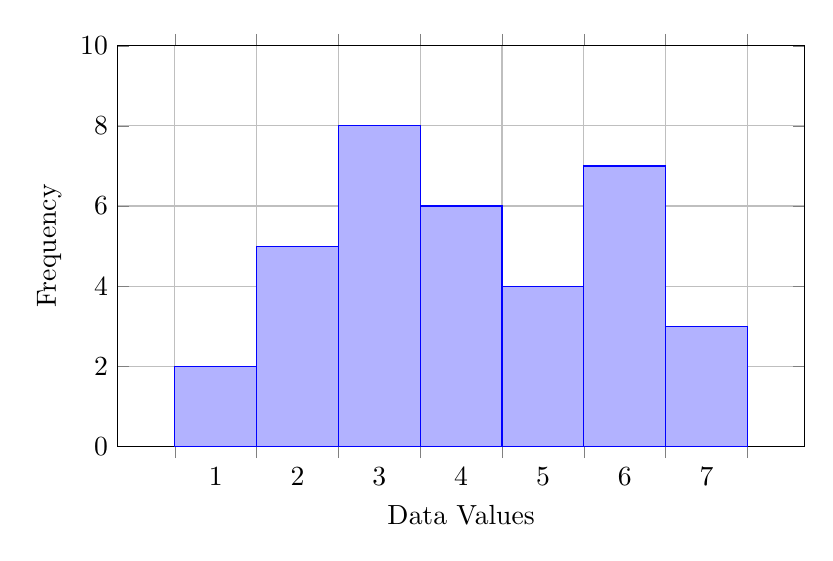
\begin{tikzpicture}
\begin{axis}[
    ybar interval,
    width=0.85\textwidth,
    height=0.55\textwidth,
    xlabel={Data Values},
    ylabel={Frequency},
    xtick={1,2,3,4,5,6,7,8},
    ymin=0,
    ymax=10,
    grid=major,
    bar width=1.0
]
\addplot coordinates {
    (1,2)
    (2,5)
    (3,8)
    (4,6)
    (5,4)
    (6,7)
    (7,3)
    (8,1)
};
\end{axis}
\end{tikzpicture}
\end{frame}
\begin{frame}{Skewness}

Skewness measures the \textbf{asymmetry} of a distribution.

\begin{block}{Symmetric}
\[
\text{Mean}\approx\text{Median}
\]
\end{block}

\begin{block}{Positive / Right Skew}
The distribution has a longer right tail.

Typically:

\[
\text{Mean}>\text{Median}
\]
\end{block}

\begin{block}{Negative / Left Skew}
The distribution has a longer left tail.

Typically:

\[
\text{Mean}<\text{Median}
\]
\end{block}
\end{frame}

\begin{frame}{Skewness}

\centering
\textbf{Skewness measures the asymmetry of a probability distribution.}

\vspace{0.3cm}

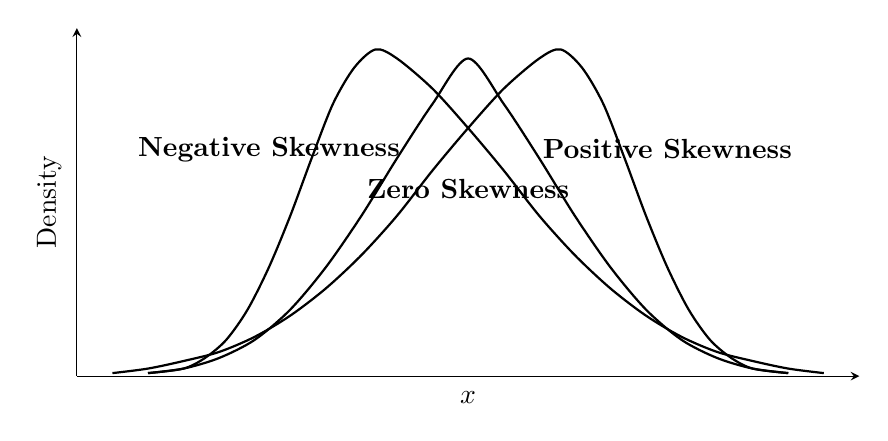
\begin{tikzpicture}
\begin{axis}[
    width=0.95\textwidth,
    height=6cm,
    axis lines=left,
    xmin=-5.5,
    xmax=5.5,
    ymin=0,
    ymax=1.15,
    xtick=\empty,
    ytick=\empty,
    xlabel={$x$},
    ylabel={Density},
    clip=false
]

\addplot[
    thick,
    smooth
]
coordinates {
(-5.0,0.01) (-4.5,0.025) (-4.0,0.05) (-3.5,0.08)
(-3.0,0.13) (-2.5,0.20) (-2.0,0.29) (-1.5,0.40)
(-1.0,0.53) (-0.5,0.68) (0,0.82) (0.5,0.95)
(1.0,1.05) (1.3,1.08) (1.6,1.02) (1.9,0.90)
(2.2,0.72) (2.5,0.53) (2.8,0.36) (3.1,0.22)
(3.4,0.12) (3.7,0.06) (4.0,0.025) (4.5,0.01)
};

\addplot[
    thick,
    smooth
]
coordinates {
(-4.5,0.01) (-4.0,0.025) (-3.5,0.06) (-3.0,0.12)
(-2.5,0.22) (-2.0,0.36) (-1.5,0.53) (-1.0,0.72)
(-0.5,0.90) (0,1.05) (0.5,0.90) (1.0,0.72)
(1.5,0.53) (2.0,0.36) (2.5,0.22) (3.0,0.12)
(3.5,0.06) (4.0,0.025) (4.5,0.01)
};

\addplot[
    thick,
    smooth
]
coordinates {
(-4.5,0.01) (-4.0,0.025) (-3.7,0.06) (-3.4,0.12)
(-3.1,0.22) (-2.8,0.36) (-2.5,0.53) (-2.2,0.72)
(-1.9,0.90) (-1.6,1.02) (-1.3,1.08) (-1.0,1.05)
(-0.5,0.95) (0,0.82) (0.5,0.68) (1.0,0.53)
(1.5,0.40) (2.0,0.29) (2.5,0.20) (3.0,0.13)
(3.5,0.08) (4.0,0.05) (4.5,0.025) (5.0,0.01)
};

\node at (axis cs:-2.8,0.75) {\textbf{Negative Skewness}};
\node at (axis cs:0,0.62) {\textbf{Zero Skewness}};
\node at (axis cs:2.8,0.75) {\textbf{Positive Skewness}};

\end{axis}
\end{tikzpicture}

\vspace{-0.1cm}

\begin{columns}

\begin{column}{0.32\textwidth}
\centering
\textbf{Negative Skewness}\\
Long left tail
\end{column}

\begin{column}{0.32\textwidth}
\centering
\textbf{Zero Skewness}\\
Symmetric distribution
\end{column}

\begin{column}{0.32\textwidth}
\centering
\textbf{Positive Skewness}\\
Long right tail
\end{column}

\end{columns}

\vspace{0.2cm}

\[
\text{Skewness}<0
\qquad
\text{Skewness}=0
\qquad
\text{Skewness}>0
\]

\end{frame}
\begin{frame}{Kurtosis}

Kurtosis describes aspects of the \textbf{tail heaviness} of a
distribution.

One population definition is:

\[
\boxed{
\text{Kurtosis}
=
\frac{E[(X-\mu)^4]}{\sigma^4}
}
\]

For a normal distribution:

\[
\text{Kurtosis}=3
\]

Excess kurtosis is:

\[
\boxed{
\text{Excess Kurtosis}
=
\text{Kurtosis}-3
}
\]

Therefore, normal distribution has excess kurtosis:

\[
0
\]
\end{frame}
\begin{frame}{Kurtosis}

\centering
\textbf{Kurtosis describes the heaviness of the tails of a distribution.}

\vspace{0.3cm}

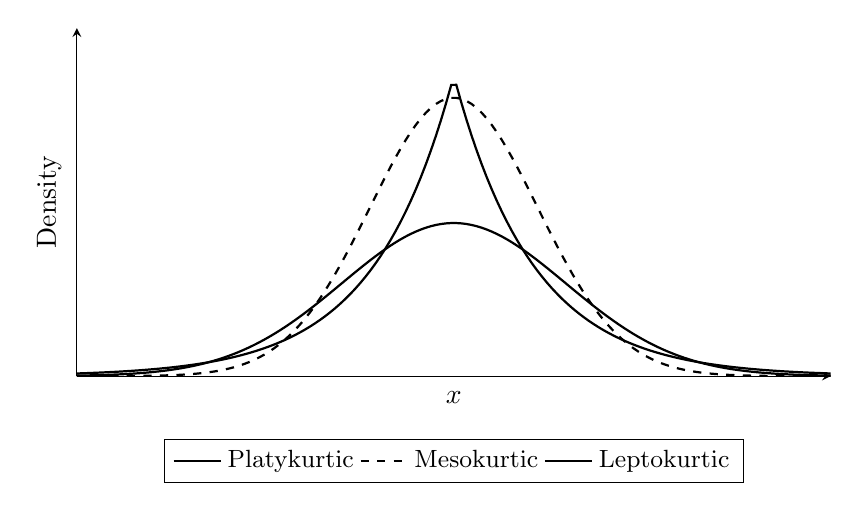
\begin{tikzpicture}
\begin{axis}[
    width=0.92\textwidth,
    height=6cm,
    axis lines=left,
    xmin=-4.5,
    xmax=4.5,
    ymin=0,
    ymax=1.25,
    xtick=\empty,
    ytick=\empty,
    xlabel={$x$},
    ylabel={Density},
    samples=150,
    legend style={
        at={(0.5,-0.18)},
        anchor=north,
        legend columns=3,
        font=\small
    }
]

\addplot[
    thick,
    domain=-4.5:4.5
]
{0.55*exp(-0.28*x^2)};
\addlegendentry{Platykurtic}

\addplot[
    thick,
    dashed,
    domain=-4.5:4.5
]
{exp(-x^2/2)};
\addlegendentry{Mesokurtic}

\addplot[
    thick,
    domain=-4.5:4.5
]
{1.08*exp(-1.05*abs(x))};
\addlegendentry{Leptokurtic}

\end{axis}
\end{tikzpicture}

\vspace{0.1cm}

\begin{columns}

\begin{column}{0.32\textwidth}
\centering
\textbf{Platykurtic}\\
Flatter distribution\\
Light tails\\
Excess kurtosis $<0$
\end{column}

\begin{column}{0.32\textwidth}
\centering
\textbf{Mesokurtic}\\
Normal-like distribution\\
Moderate tails\\
Excess kurtosis $=0$
\end{column}

\begin{column}{0.32\textwidth}
\centering
\textbf{Leptokurtic}\\
More peaked distribution\\
Heavy tails\\
Excess kurtosis $>0$
\end{column}

\end{columns}

\vspace{0.2cm}

\[
\text{Excess Kurtosis}=\text{Kurtosis}-3
\]

\end{frame}


\begin{frame}{Sample Mean and Sample Variance}

For a sample:

\[
X_1,X_2,\ldots,X_n
\]

the sample mean is:

\[
\boxed{
\bar X=
\frac{1}{n}\sum_{i=1}^{n}X_i
}
\]

The sample variance is:

\[
\boxed{
S^2=
\frac{1}{n-1}
\sum_{i=1}^{n}(X_i-\bar X)^2
}
\]

The sample mean estimates the population mean $\mu$ and
the sample variance estimates the population variance $\sigma^2$.
\end{frame}

\begin{frame}{Order Statistics}
Suppose the observations are:
\[
8,\;3,\;10,\;5,\;2
\]
After sorting:
\[
2,\;3,\;5,\;8,\;10
\]
These ordered observations are called \textbf{order statistics}.
They are denoted by:
\[
X_{(1)},X_{(2)},\ldots,X_{(n)}
\]
where:
\[
X_{(1)}=\text{smallest observation}
\]
and
\[
X_{(n)}=\text{largest observation}
\]
Order statistics are used to calculate medians, quartiles,
percentiles, minimum and maximum values.
\end{frame}

\begin{frame}{Sample Covariance}

Covariance measures the direction of the linear relationship
between two variables.

For variables $X$ and $Y$:

\[
\boxed{
S_{XY}
=
\frac{1}{n-1}
\sum_{i=1}^{n}
(X_i-\bar X)(Y_i-\bar Y)
}
\]

\begin{block}{Interpretation}
\begin{itemize}
    \item $S_{XY}>0$: variables tend to increase together.
    \item $S_{XY}<0$: one tends to increase as the other decreases.
    \item $S_{XY}\approx0$: little linear association.
\end{itemize}
\end{block}

Zero covariance does not necessarily imply that there is
no relationship; a nonlinear relationship may exist.
\end{frame}

\begin{frame}{Sample Covariance Matrix}
For variables:
\[
X_1,X_2,\ldots,X_p
\]
the sample covariance matrix is:
\[
\boxed{
S=
\begin{bmatrix}
S_{11} & S_{12} & \cdots & S_{1p}\\
S_{21} & S_{22} & \cdots & S_{2p}\\
\vdots & \vdots & \ddots & \vdots\\
S_{p1} & S_{p2} & \cdots & S_{pp}
\end{bmatrix}
}
\]
where:
\[
S_{ii}=\text{Variance of }X_i
\]
and
\[
S_{ij}=\text{Covariance of }X_i\text{ and }X_j
\]
Since:
\[
S_{ij}=S_{ji}
\]
the covariance matrix is symmetric.
\end{frame}

\begin{frame}{Example: Covariance Matrix}

Consider:

\[
S=
\begin{bmatrix}
4 & 2 & -1\\
2 & 9 & 3\\
-1 & 3 & 16
\end{bmatrix}
\]

Therefore:

\begin{itemize}
    \item $\operatorname{Var}(X_1)=4$
    \item $\operatorname{Var}(X_2)=9$
    \item $\operatorname{Var}(X_3)=16$
    \item $\operatorname{Cov}(X_1,X_2)=2$
    \item $\operatorname{Cov}(X_1,X_3)=-1$
    \item $\operatorname{Cov}(X_2,X_3)=3$
\end{itemize}

Covariance matrices are widely used in:

\[
\boxed{\text{Machine Learning, PCA, Multivariate Statistics}}
\]
\end{frame}

\begin{frame}{Frequentist Statistics}

Frequentist statistics is a framework for statistical inference
based on the behavior of statistical procedures under
\textbf{repeated sampling}.

In the frequentist framework:

\begin{itemize}
    \item Population parameters are fixed but unknown.
    \item Data are treated as random.
    \item Samples are used to make conclusions about populations.
\end{itemize}

Example:

\[
X_1,X_2,\ldots,X_n
\]

are observations used to estimate the unknown population mean $\mu$.
\end{frame}

\begin{frame}{Sampling}

Sampling is the process of selecting observations from a population.

\begin{center}
\[
\boxed{\text{Population}}
\rightarrow
\boxed{\text{Sampling}}
\rightarrow
\boxed{\text{Sample}}
\rightarrow
\boxed{\text{Inference}}
\]
\end{center}

\textbf{Population:} Complete set of objects or individuals of interest.

\textbf{Sample:} A subset selected from the population.

Example:

\begin{itemize}
    \item Population: All students in a university.
    \item Sample: 100 students selected for a survey.
\end{itemize}
\end{frame}

\begin{frame}{Types of Sampling}

\begin{block}{Simple Random Sampling}
Every member has an equal or known chance of selection.
\end{block}

\begin{block}{Stratified Sampling}
Population is divided into groups called strata and samples
are taken from each group.
\end{block}

\begin{block}{Systematic Sampling}
Every $k$-th observation is selected after a random starting point.
\end{block}

\begin{block}{Cluster Sampling}
Population is divided into clusters and some clusters are selected.
\end{block}
\end{frame}

\begin{frame}{Parameter and Statistic}

\textbf{Parameter:}

A numerical characteristic of a population.

\[
\mu=\text{Population mean}
\]

\[
\sigma^2=\text{Population variance}
\]

\vspace{0.3cm}

\textbf{Statistic:}

A quantity calculated from sample data.

\[
\bar X=\text{Sample mean}
\]

\[
S^2=\text{Sample variance}
\]

\vspace{0.3cm}

\begin{center}
\[
\boxed{\text{Sample Statistic}\rightarrow\text{Estimate of Population Parameter}}
\]
\end{center}
\end{frame}

\begin{frame}{Statistical Estimation}

Estimation is the process of using sample data to estimate
an unknown population parameter.

\begin{block}{Point Estimation}
Provides a single value.

\[
\hat{\mu}=\bar X
\]
\end{block}

\begin{block}{Interval Estimation}
Provides a range of plausible values.

\[
L<\mu<U
\]
\end{block}

The estimator $\hat{\theta}$ is calculated from sample data
and is used to estimate the unknown parameter $\theta$.
\end{frame}

\begin{frame}{Mean Square Error}

Mean Square Error (MSE) measures the average squared difference
between an estimator and the true parameter.

For estimator $\hat{\theta}$:

\[
\boxed{
MSE(\hat{\theta})
=
E[(\hat{\theta}-\theta)^2]
}
\]

MSE can be decomposed as:

\[
\boxed{
MSE(\hat{\theta})
=
\operatorname{Var}(\hat{\theta})
+
[\operatorname{Bias}(\hat{\theta})]^2
}
\]

where:

\[
\operatorname{Bias}(\hat{\theta})
=
E[\hat{\theta}]-\theta
\]

A smaller MSE generally indicates an estimator with better
overall accuracy under the chosen criterion.
\end{frame}

\begin{frame}{Consistency}

An estimator is \textbf{consistent} if it approaches the true
population parameter as the sample size increases.

For estimator $\hat{\theta}_n$:

\[
\boxed{
\hat{\theta}_n
\xrightarrow{P}
\theta
\quad\text{as}\quad n\rightarrow\infty
}
\]

This means:

\begin{center}
\text{More data}
$\rightarrow$
\text{Estimator becomes increasingly close to the true parameter}
\end{center}

Under standard conditions, the sample mean is a consistent
estimator of the population mean.
\end{frame}

\begin{frame}{Confidence Intervals}

A confidence interval is an interval calculated from sample data
using a procedure designed to contain an unknown population
parameter at a specified long-run frequency.

If population standard deviation $\sigma$ is known:

\[
\boxed{
\bar X
\pm
z_{\alpha/2}
\frac{\sigma}{\sqrt n}
}
\]

For a 95\% confidence interval:

\[
\boxed{
\bar X
\pm
1.96\frac{\sigma}{\sqrt n}
}
\]

If $\sigma$ is unknown:

\[
\boxed{
\bar X
\pm
t_{\alpha/2,n-1}
\frac{S}{\sqrt n}
}
\]
\end{frame}

\begin{frame}{Interpretation of a 95\% Confidence Interval}

A 95\% confidence procedure means:

\begin{center}
\textbf{If we repeatedly take samples and construct intervals
using the same method, approximately 95\% of those intervals
will contain the true parameter.}
\end{center}

\vspace{0.5cm}

It does \textbf{not} strictly mean that there is a 95\% probability
that the fixed population parameter lies inside the particular
interval that has already been calculated.
\end{frame}

\begin{frame}{Parametric Model Estimation}
A parametric model assumes that the population distribution
belongs to a specified family described by a finite number
of parameters.
Example:
\[
X\sim N(\mu,\sigma^2)
\]
The parameters are:
\[
\theta=(\mu,\sigma^2)
\]
They can be estimated using sample data:
\[
\hat{\mu}=\bar X
\]
\[
\hat{\sigma}^2=S^2
\]
Common parametric models include:
\begin{itemize}
    \item Normal distribution
    \item Binomial distribution
    \item Poisson distribution
    \item Exponential distribution
\end{itemize}
\end{frame}

\begin{frame}{Maximum Likelihood Estimation}

Maximum Likelihood Estimation (MLE) is an important method
of parametric estimation.
For observations:

\[
X_1,X_2,\ldots,X_n
\]
the likelihood function is:
\[
\boxed{
L(\theta)
=
\prod_{i=1}^{n}f(x_i|\theta)
}
\]

The maximum likelihood estimator is:
\[
\boxed{
\hat{\theta}
=
\arg\max_{\theta}L(\theta)
}
\]
Often the log-likelihood is maximized instead:

\[
\boxed{
\hat{\theta}
=
\arg\max_{\theta}\log L(\theta)
}
\]
\end{frame}

\begin{frame}{MLE: Basic Process}
\begin{center}
\[
\boxed{\text{Observed Data}}
\]
$\downarrow$
\[
\boxed{\text{Choose Statistical Model}}
\]
$\downarrow$
\[
\boxed{\text{Construct Likelihood}}
\]
$\downarrow$
\[
\boxed{\text{Maximize Likelihood}}
\]
$\downarrow$
\[
\boxed{\text{Estimated Parameters}}
\]
\end{center}
\end{frame}

\begin{frame}{Non-Parametric Model Estimation}

Non-parametric methods make fewer assumptions about the exact
form of the population distribution.

Instead of assuming:

\[
X\sim N(\mu,\sigma^2)
\]

the distribution can be estimated more flexibly from the data.

Examples:

\begin{itemize}
    \item Empirical distribution
    \item Histogram-based estimation
    \item Kernel density estimation
    \item Rank-based methods
\end{itemize}
\end{frame}

\begin{frame}{Kernel Density Estimation}

Kernel Density Estimation (KDE) estimates the probability
density function from observations.

\[
\boxed{
\hat f_h(x)
=
\frac{1}{nh}
\sum_{i=1}^{n}
K\left(
\frac{x-X_i}{h}
\right)
}
\]

where:

\begin{itemize}
    \item $K$ = Kernel function
    \item $h$ = Bandwidth
    \item $n$ = Number of observations
\end{itemize}

The bandwidth controls the smoothness of the estimated density.
\end{frame}

\begin{frame}{Parametric vs Non-Parametric}

\begin{center}
\begin{tabular}{>{\bfseries}m{3.3cm} m{3.5cm} m{3.5cm}}
\toprule
Feature & Parametric & Non-Parametric\\
\midrule
Assumptions & Specific distributional family & Fewer distributional assumptions\\
Flexibility & Lower & Higher\\
Parameters & Finite-dimensional & Not restricted to a fixed finite-dimensional form\\
Example & Normal model & KDE\\
Data & Can work well with smaller samples if model is appropriate & Often needs more data for good accuracy\\
\bottomrule
\end{tabular}
\end{center}
\end{frame}

\begin{frame}{Descriptive Statistics: Overall View}
\begin{center}
\[
\boxed{\text{DATA}}
\]
$\downarrow$
\[
\boxed{\text{Organize and Summarize}}
\]
$\downarrow$
\[
\boxed{
\begin{array}{c}
\text{Central Tendency}\\
\text{Dispersion}\\
\text{Distribution Shape}
\end{array}
}
\]

$\downarrow$

\[
\boxed{\text{Describe the Dataset}}
\]
\end{center}
\end{frame}

\begin{frame}{Frequentist Statistics: Overall View}
\begin{center}
\[
\boxed{\text{POPULATION}}
\]
$\downarrow$
\[
\boxed{\text{SAMPLING}}
\]
$\downarrow$
\[
\boxed{\text{SAMPLE}}
\]
$\downarrow$
\[
\boxed{\text{STATISTICS}}
\]
$\downarrow$
\[
\boxed{\text{ESTIMATION}}
\]
$\downarrow$
\[
\boxed{\text{INFERENCE}}
\]
\end{center}

Important concepts:
\[
\text{MSE,\ Consistency,\ Confidence Intervals,\ Parametric and Non-Parametric Estimation}
\]
\end{frame}

\begin{frame}{Complete Connection}

\begin{center}
\Large
\[
\boxed{
\text{Data}
\rightarrow
\text{Information}
\rightarrow
\text{Knowledge}
\rightarrow
\text{Intelligence}
}
\]
\end{center}

\vspace{0.4cm}

\[
\boxed{
\text{Statistics}
\rightarrow
\text{Analyze Data}
\rightarrow
\text{Extract Information}
\rightarrow
\text{Support Knowledge}
\rightarrow
\text{Decision Making}
}
\]

\vspace{0.4cm}

AI combines:

\[
\boxed{
\text{Data + Algorithms + Models}
\rightarrow
\text{Learning + Reasoning + Decision Making}
}
\]

\end{frame}

\begin{frame}{Applications in AI and Machine Learning}

Statistical concepts are fundamental to AI and Machine Learning.

\begin{itemize}
    \item Mean and variance help understand datasets.
    \item Covariance helps identify relationships between features.
    \item Covariance matrices are used in PCA.
    \item Histograms help understand feature distributions.
    \item Skewness and kurtosis describe distribution shape.
    \item Sampling provides training and testing data.
    \item Estimation is used to learn model parameters.
    \item MSE is widely used as a loss function in regression.
    \item Confidence intervals quantify uncertainty.
    \item Parametric and non-parametric methods provide different approaches to modelling data.
\end{itemize}
\end{frame}

\begin{frame}{Conclusion}

\begin{itemize}
    \item \textbf{Descriptive statistics} summarizes and describes observed data.
    \item Measures of central tendency describe the center of data.
    \item Measures of dispersion describe the spread.
    \item IQR, box plots and histograms help understand distributions and outliers.
    \item Skewness and kurtosis describe distribution shape.
    \item Covariance describes relationships between variables.
    \item \textbf{Frequentist statistics} uses samples to make inferences about populations.
    \item Estimation, MSE, consistency and confidence intervals are important tools of inference.
    \item Parametric and non-parametric methods provide different approaches to statistical modelling.
    \item These concepts form an important statistical foundation for AI and Machine Learning.
\end{itemize}

\end{frame}

\begin{frame}
\begin{center}
\Huge
\textbf{Thank You}
\end{center}
\end{frame}

\end{document}